\documentclass[12pt, a4paper]{report}
\usepackage[top=3cm,left=3cm,right=2cm,bottom=2cm]{geometry}
\linespread{1.3}
\setlength{\parindent}{1.25cm}
\usepackage{indentfirst}
\usepackage[utf8]{inputenc}
\usepackage[brazil]{babel}
\usepackage{amsmath}
\usepackage{amsthm}
\usepackage{amsfonts}
\usepackage{amssymb}
\usepackage{graphicx}
\usepackage{color}
\usepackage{multicol}
\usepackage[normalem]{ulem}
\usepackage{wrapfig}
\usepackage{caption}
\usepackage{fancybox}
\usepackage[pdfstartview=FitH]{hyperref}
\usepackage{subfigure}
\bibliographystyle{plain}
\usepackage{algorithm}
\usepackage{algpseudocode}
\usepackage{float}


\graphicspath{{Figuras/}{resultados/}}

\renewcommand{\theenumii}{\alph{enumii}}
\DeclareMathOperator{\sen}{sen}
\DeclareMathOperator{\tg}{tg}
\DeclareMathOperator{\arctg}{arctg}
\DeclareMathOperator{\cotg}{cotg}
\DeclareMathOperator{\agm}{agm}

\newtheorem{thm}{Teorema}[section]
\newtheorem{dfn}{Definição}[section]
\newtheorem{prob}{Problema}[section]
\newtheorem{cor}{Corolário}[section]
\newtheorem{prop}{Proposição}[section]
\newtheorem{lem}{Lema} [section]

\newcounter{contar}
%  #endregion preâmbulo

% #region Variáveis 
\newcommand{\nomeUniversidade}{Universidade Federal da Bahia}
\newcommand{\nomeInstituto}{Instituto de Computação}
\newcommand{\nomeCurso}{MATA53 - Teoria dos grafos}
\newcommand{\nomeProfessor}{Islame Felipe da Costa Fernandes}
\newcommand{\nomeGrupo}{\sc{\large{Antoniel Magalhães}} \\
\sc{\large{João Leahy}} \\
\sc{\large{Luis Felipe}}}
\newcommand{\titulo}{\sc{\Large{Problema de Colocação Ótima de Câmeras de Segurança no bairro da Ondina}}}
% #endregion Variáveis 

\begin{document}

% #region capa
\pagestyle{empty}
\begin{center}

\includegraphics[height=2.5cm]{UFBA.jpg}
\hspace{2cm}
\end{center}

\begin{center}
\sc{\large{\nomeUniversidade}} \\
\sc{\large{\nomeInstituto}} \\
\sc{\small{\nomeCurso}} \\

\vspace{4cm}

\titulo

\vspace{4.5cm}

\nomeGrupo


\vspace{5.5cm}

\textbf{Salvador - Bahia} \\
\today
\end{center}
% #endregion capa

% #region folha de rosto
\newpage
\begin{center}
\titulo

\vspace{4cm}

\nomeGrupo
\end{center}

\vspace{4cm}

\begin{flushright}
\begin{minipage}{8.6cm}
Projeto final entregue ao professor \nomeProfessor\ 
como método avaliativo da disciplina \nomeCurso


\end{minipage}
\end{flushright}
 
\vspace{8cm}


\begin{center}
\textbf{Salvador - Bahia} \\
\today
\end{center}

% #endregion folha de rosto

% #region Índice
\newpage
\tableofcontents
\thispagestyle{empty}
\newpage
\setcounter{page}{1}
\pagestyle{plain}
% #endregion Índice


\chapter{Introdução}

\section{Contextualização e Motivação}
A teoria dos grafos oferece um poderoso conjunto de ferramentas matemáticas para modelar e resolver problemas complexos de otimização em redes. No contexto da segurança pública, o problema de posicionamento de câmeras de vigilância pode ser elegantemente modelado como um problema de cobertura mínima de vértices (Minimum Vertex Cover). Nesta abordagem, os vértices do grafo representam possíveis localizações de câmeras, e as arestas representam as áreas que precisam ser monitoradas. O bairro de Ondina, em Salvador, apresenta um cenário ideal para aplicação deste conceito, por concentrar pontos estratégicos como a Universidade Federal da Bahia, estabelecimentos comerciais, hotéis e áreas residenciais, além de um intenso fluxo turístico devido às suas praias.

\section{Justificativa}
A aplicação de conceitos fundamentais da teoria dos grafos, como cobertura de vértices, dominação e problemas de localização de facilidades, fornece uma base teórica sólida para abordar o problema de posicionamento de câmeras. Este trabalho permite explorar na prática diversos algoritmos e técnicas estudados na disciplina MATA53 - Teoria dos Grafos, como algoritmos gulosos, programação dinâmica e métodos de otimização em grafos. A escolha do bairro de Ondina como objeto de estudo possibilita uma aplicação real desses conceitos, contribuindo tanto para o aprendizado acadêmico quanto para uma possível solução prática de segurança pública.

\section{Objetivos do Projeto}

\subsection{Objetivo Geral}
O objetivo geral deste projeto foi desenvolver uma solução otimizada para o posicionamento de câmeras de segurança, minimizando a quantidade necessária para garantir uma cobertura total das áreas de interesse no bairro de Ondina.

\subsection{Objetivos Específicos}
\begin{itemize}
    \item Implementar diferentes algoritmos de cobertura de vértices, incluindo algoritmos gulosos e de programação dinâmica, para determinar a solução mais eficiente. A comparação entre os algoritmos foi realizada com base em critérios de eficiência e cobertura.
    \item Analisar a complexidade computacional e a eficiência dos algoritmos implementados. A análise revelou que o algoritmo guloso, embora não ótimo, ofereceu uma solução eficiente em tempo polinomial, adequada para o contexto urbano de Ondina.
    \item Avaliar a aplicabilidade das soluções teóricas em um cenário real de implementação. A modelagem do bairro de Ondina como um grafo permitiu a aplicação prática dos conceitos teóricos, resultando em uma solução viável para o problema de segurança pública.
\end{itemize}

\section{Metodologia}
\textbf{Modelagem do Problema:} O problema de localização de câmeras de segurança será abordado como um problema de \textbf{cobertura de vértices}, onde:
\begin{itemize}
    \item Os \textbf{vértices} do grafo representam os pontos de interesse a serem monitorados e os potenciais locais de instalação das câmeras.
    \item As \textbf{arestas} representam a visibilidade ou alcance de uma câmera para um determinado ponto de interesse.
\end{itemize}

\textbf{Construção do Grafo:} A região de Ondina será mapeada, identificando pontos estratégicos e possíveis locais de instalação. Um grafo será construído com base nesse mapeamento. Matrizes de adjacência ou listas de adjacência podem ser usadas para representar o grafo.

\textbf{Seleção de Algoritmos:} Serão implementados e comparados algoritmos para resolver o problema de cobertura mínima de vértices. Isso incluirá:
\begin{itemize}
    \item Algoritmos \textbf{heurísticos} para o problema de cobertura de vértices que oferecem soluções aproximadas em tempo polinomial.
    \item Algoritmos de \textbf{busca em grafos}, como busca em profundidade e largura, que podem ser úteis na identificação de conexões e componentes do grafo.
\end{itemize}


\section{Organização do Trabalho}
O projeto está estruturado de forma modular e organizada, com todo o código-fonte disponível publicamente no repositório GitHub (\url{https://github.com/antoniel/mata53-projeto-final}). A organização do trabalho segue uma abordagem sistemática, dividida em etapas bem definidas:

\subsection{Estrutura do Repositório}
O projeto está organizado em diretórios específicos, cada um com uma responsabilidade bem definida:
\begin{itemize}
    \item \texttt{scripts/}: Contém os scripts Python responsáveis pela extração, processamento e análise dos dados:
    \begin{itemize}
        \item \texttt{5\_resolve\_cobertura.py}: Implementa os algoritmos de cobertura completa e máxima
        \item \texttt{6\_visualiza\_cobertura.py}: Gera visualizações comparativas das soluções
        \item Scripts auxiliares para extração e processamento dos dados do OpenStreetMap
    \end{itemize}
    
    \item \texttt{instancias/}: Armazena os dados de entrada do problema:
    \begin{itemize}
        \item \texttt{ondina.json}: Grafo do bairro de Ondina em formato JSON, contendo nós (vértices) com coordenadas geográficas e arestas com pesos e nomes das ruas
    \end{itemize}
    
    \item \texttt{resultados/}: Contém os arquivos de saída gerados pelos algoritmos:
    \begin{itemize}
        \item \texttt{cobertura\_completa.json}: Resultado da solução de cobertura completa
        \item \texttt{cobertura\_maxima.json}: Resultado da solução de cobertura máxima
        \item \texttt{visualizacao\_cobertura.png}: Visualização comparativa das soluções
        \item \texttt{README.md}: Documentação detalhada dos resultados obtidos
    \end{itemize}
\end{itemize}

\subsection{Resultados Obtidos}
Na execução com o grafo do bairro de Ondina, obtivemos resultados significativos que demonstram a eficácia dos algoritmos implementados:

\begin{itemize}
    \item \textbf{Cobertura Completa:}
    \begin{itemize}
        \item Necessita de 80 câmeras para cobrir todos os 182 vértices do grafo
        \item Média de 2,3 vértices cobertos por câmera
        \item Garante monitoramento completo da região
    \end{itemize}
    
    \item \textbf{Cobertura Máxima:}
    \begin{itemize}
        \item Com apenas 10 câmeras, consegue cobrir 42 vértices
        \item Representa 23\% do total de vértices do grafo
        \item Média de 4,2 vértices cobertos por câmera
        \item Solução otimizada para cenários com restrição de recursos
    \end{itemize}
\end{itemize}

\begin{figure}[H]
    \centering
    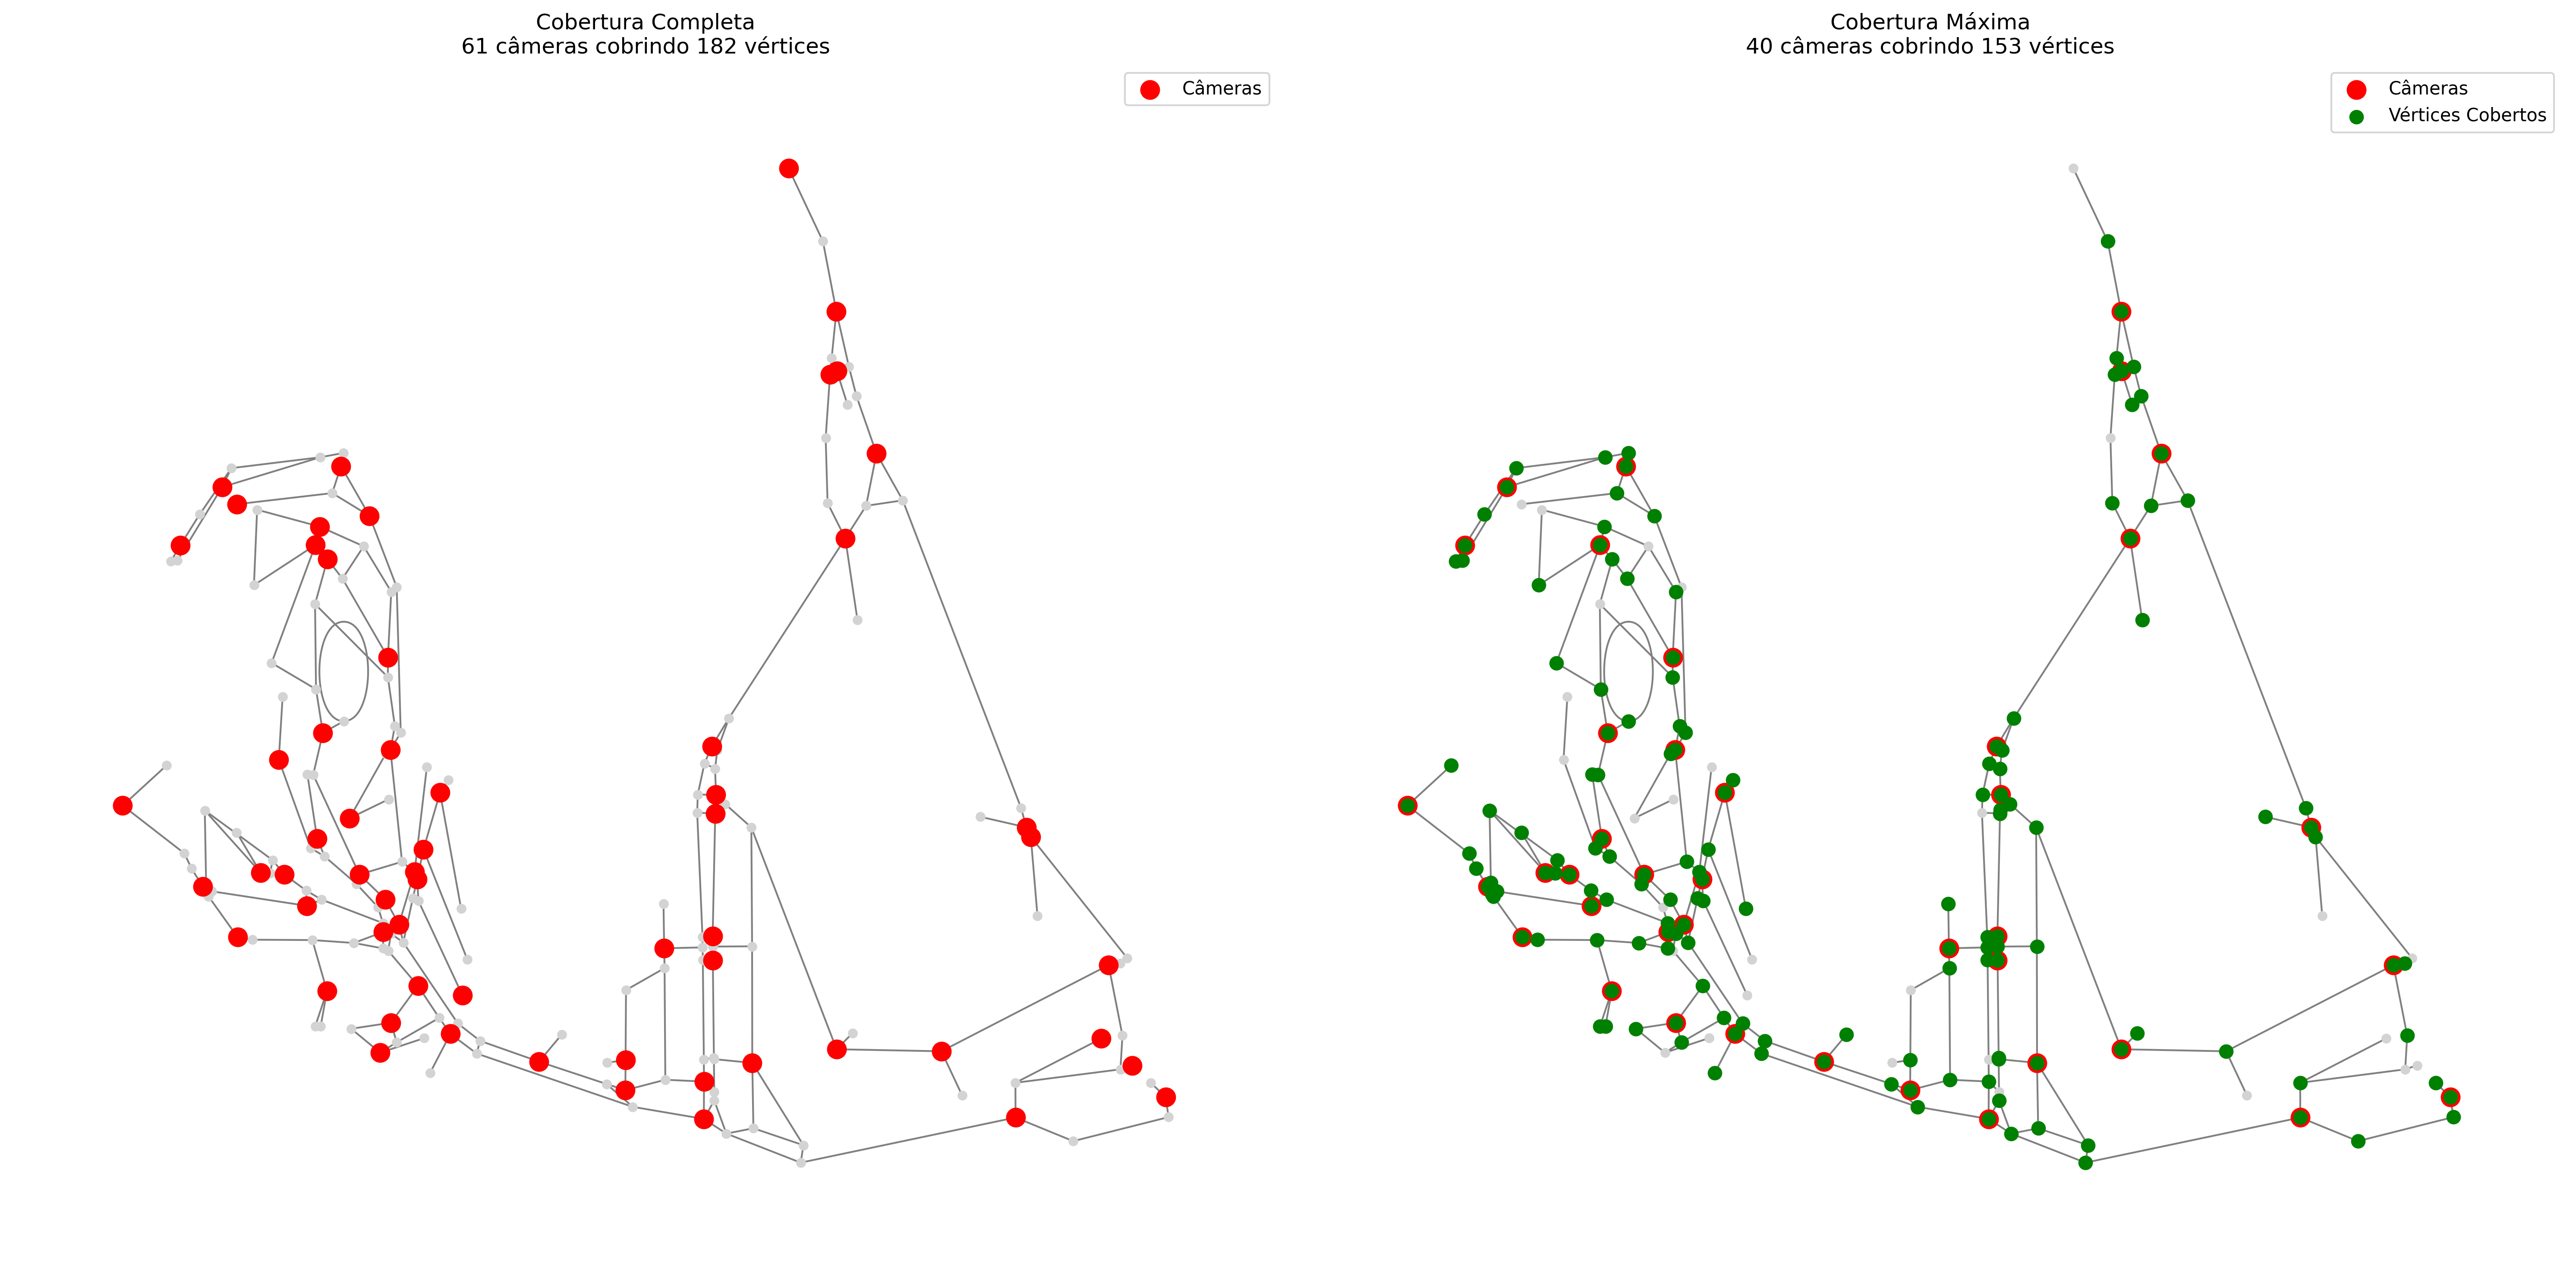
\includegraphics[width=\textwidth]{resultados/visualizacao_cobertura}
    \caption{Comparação das soluções de cobertura. À esquerda: cobertura completa com 61 câmeras cobrindo 182 vértices. À direita: cobertura máxima com 10 câmeras cobrindo 48 vértices.}
    \label{fig:visualizacao_cobertura}
\end{figure}

A Figura~\ref{fig:visualizacao_cobertura} apresenta uma comparação visual das duas soluções implementadas. Na solução de cobertura completa (esquerda), os pontos vermelhos indicam as 80 câmeras necessárias para monitorar toda a região. Na solução de cobertura máxima (direita), os pontos vermelhos mostram as 10 câmeras selecionadas, e os pontos verdes indicam os vértices cobertos por essas câmeras, demonstrando a eficiência da solução mesmo com recursos limitados.

\subsection{Documentação e Reprodutibilidade}
O projeto foi desenvolvido com foco na reprodutibilidade e facilidade de uso. Para isso, foram implementados:

\begin{itemize}
    \item Documentação detalhada no README do repositório
    \item Instruções claras para instalação de dependências via \texttt{requirements.txt}
    \item Scripts bem documentados com docstrings e comentários explicativos
    \item Geração automática de relatórios de resultados em formato markdown
    \item Logs informativos durante a execução dos algoritmos
    \item Visualizações comparativas das soluções para análise dos resultados
\end{itemize}

Os capítulos seguintes detalham cada aspecto do trabalho, desde a fundamentação teórica até a análise dos resultados obtidos, apresentando uma visão completa do desenvolvimento e das conclusões alcançadas.

\chapter{Trabalhos Correlatos}
% #TODO: melhorar o capítulo
O problema de cobertura mínima de vértices tem sido extensivamente estudado na literatura, tanto em sua forma teórica quanto em aplicações práticas. Esta seção apresenta uma revisão dos principais trabalhos relacionados, focando em resultados teóricos fundamentais e aplicações similares ao nosso problema de posicionamento de câmeras.

\chapter{Descrição Formal do Problema}

\section{Formalização}
O problema é formalizado como um grafo \(G = (V, E)\), onde os vértices \(V\) representam locais possíveis para câmeras e as arestas \(E\) representam conexões entre pontos que precisam ser monitorados. O objetivo é encontrar o menor subconjunto de vértices \(C \subseteq V\) tal que cada aresta em \(E\) é incidente a pelo menos um vértice em \(C\).

\section{Restrições do Problema}
As restrições incluem orçamento limitado, número máximo de câmeras, e a necessidade de cobrir áreas prioritárias.

\section{Função Objetivo}
A função objetivo é minimizar o número de câmeras necessárias para cobrir todas as ruas, garantindo que cada rua seja monitorada por pelo menos uma câmera.

\section{Modelagem em Grafos}

A modelagem da malha viária do bairro de Ondina, em Salvador, foi realizada utilizando grafos extraídos do OpenStreetMap. O grafo representa as ruas do bairro, onde os nós correspondem a pontos geográficos (latitude e longitude), e as arestas conectam esses pontos, representando as ruas ou caminhos disponíveis.

\section{Extração, Processamento e Modelagem do Grafo}

A construção do grafo que modela a malha viária do bairro de Ondina em Salvador foi realizada a partir de dados extraídos do OpenStreetMap (OSM). Este processo envolveu múltiplas etapas, desde a coleta dos dados geográficos até a simplificação e ajuste do grafo para adequação ao problema em análise.

\subsection{Extração de Dados}

Os dados do OSM, uma base colaborativa que fornece informações detalhadas sobre vias. Passaram por algumas transformações para obtermos apenas as informações necessárias.

A Figura~\ref{fig:ondina_ruas} apresenta a visualização inicial das ruas do bairro de Ondina, com base nos dados brutos extraídos do OSM.

\begin{figure}[H]
    \centering
    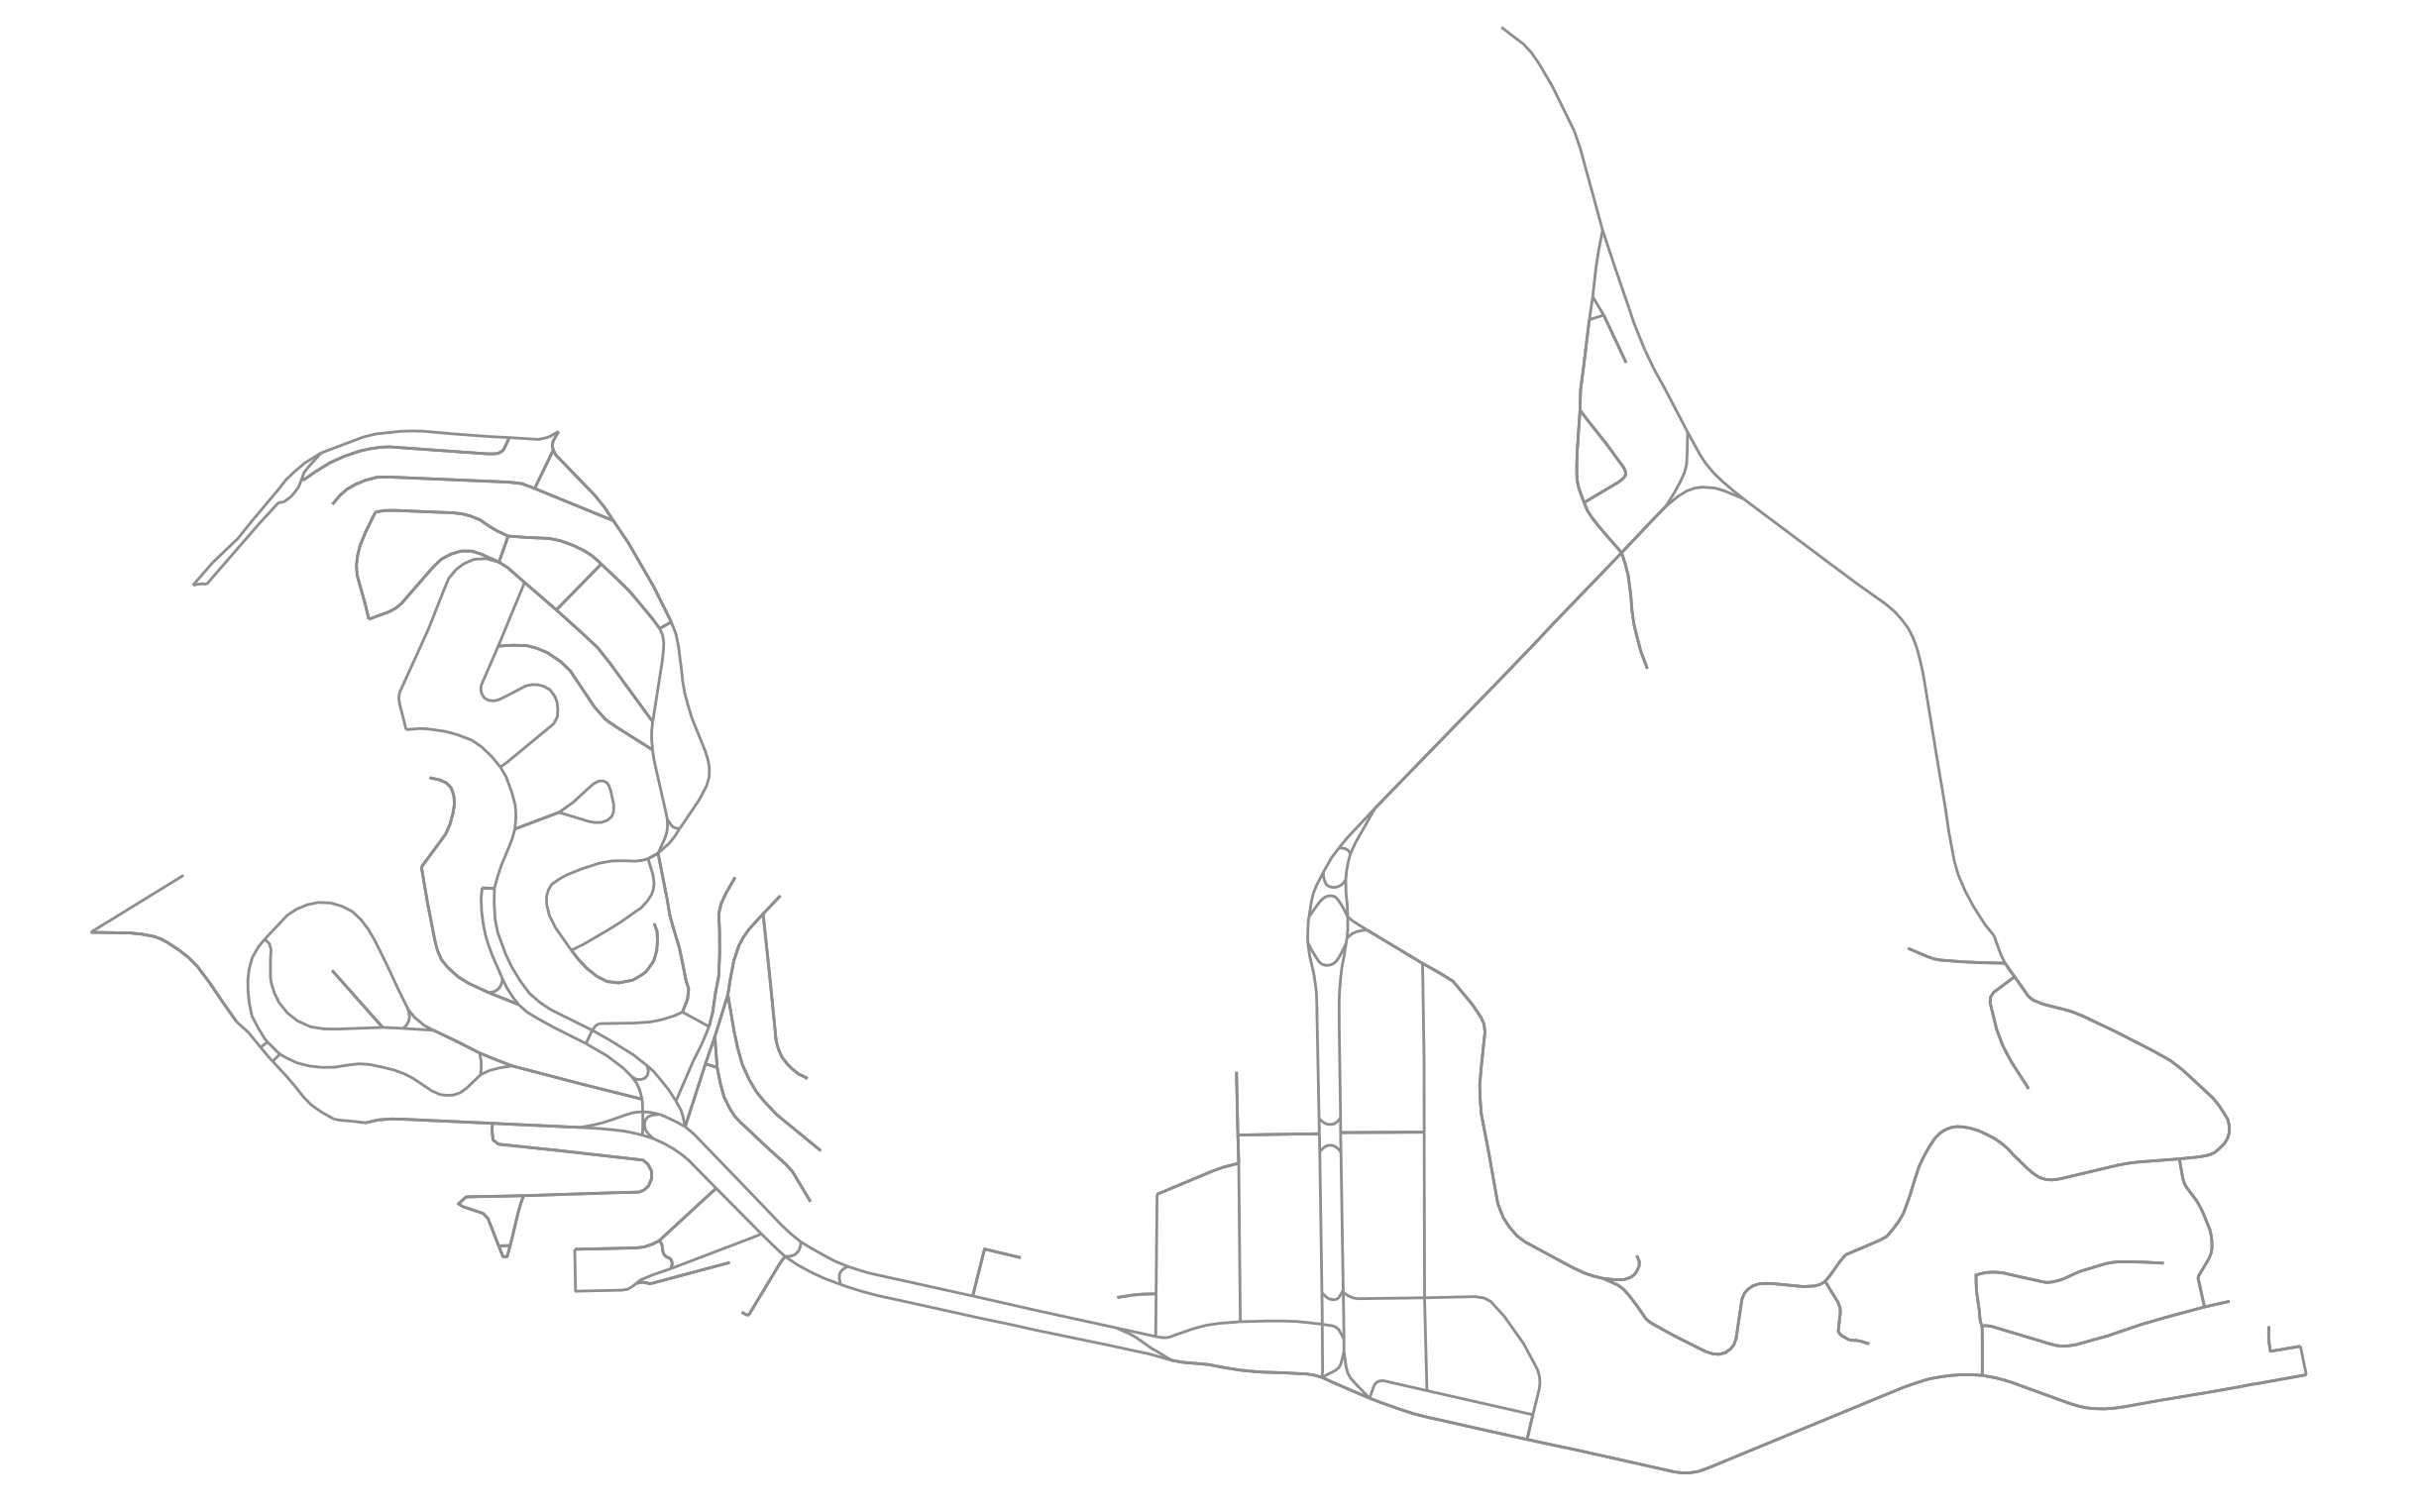
\includegraphics[width=\textwidth]{visualizacao_inicial}
    \caption{Visualização inicial das ruas do bairro de Ondina.}
    \label{fig:ondina_ruas}
\end{figure}

\subsection{Processamento e Construção do Grafo}

Após a extração dos dados, foi realizado o mapeamento para um grafo. Nesta etapa, os nós foram associados aos pontos geográficos, enquanto as arestas representaram as conexões entre eles, sendo atribuído um peso correspondente à distância entre os pontos. A Figura~\ref{fig:ondina_grafo_bruto} mostra a visualização das ruas com os vértices associados.

\begin{figure}[H]
    \centering
    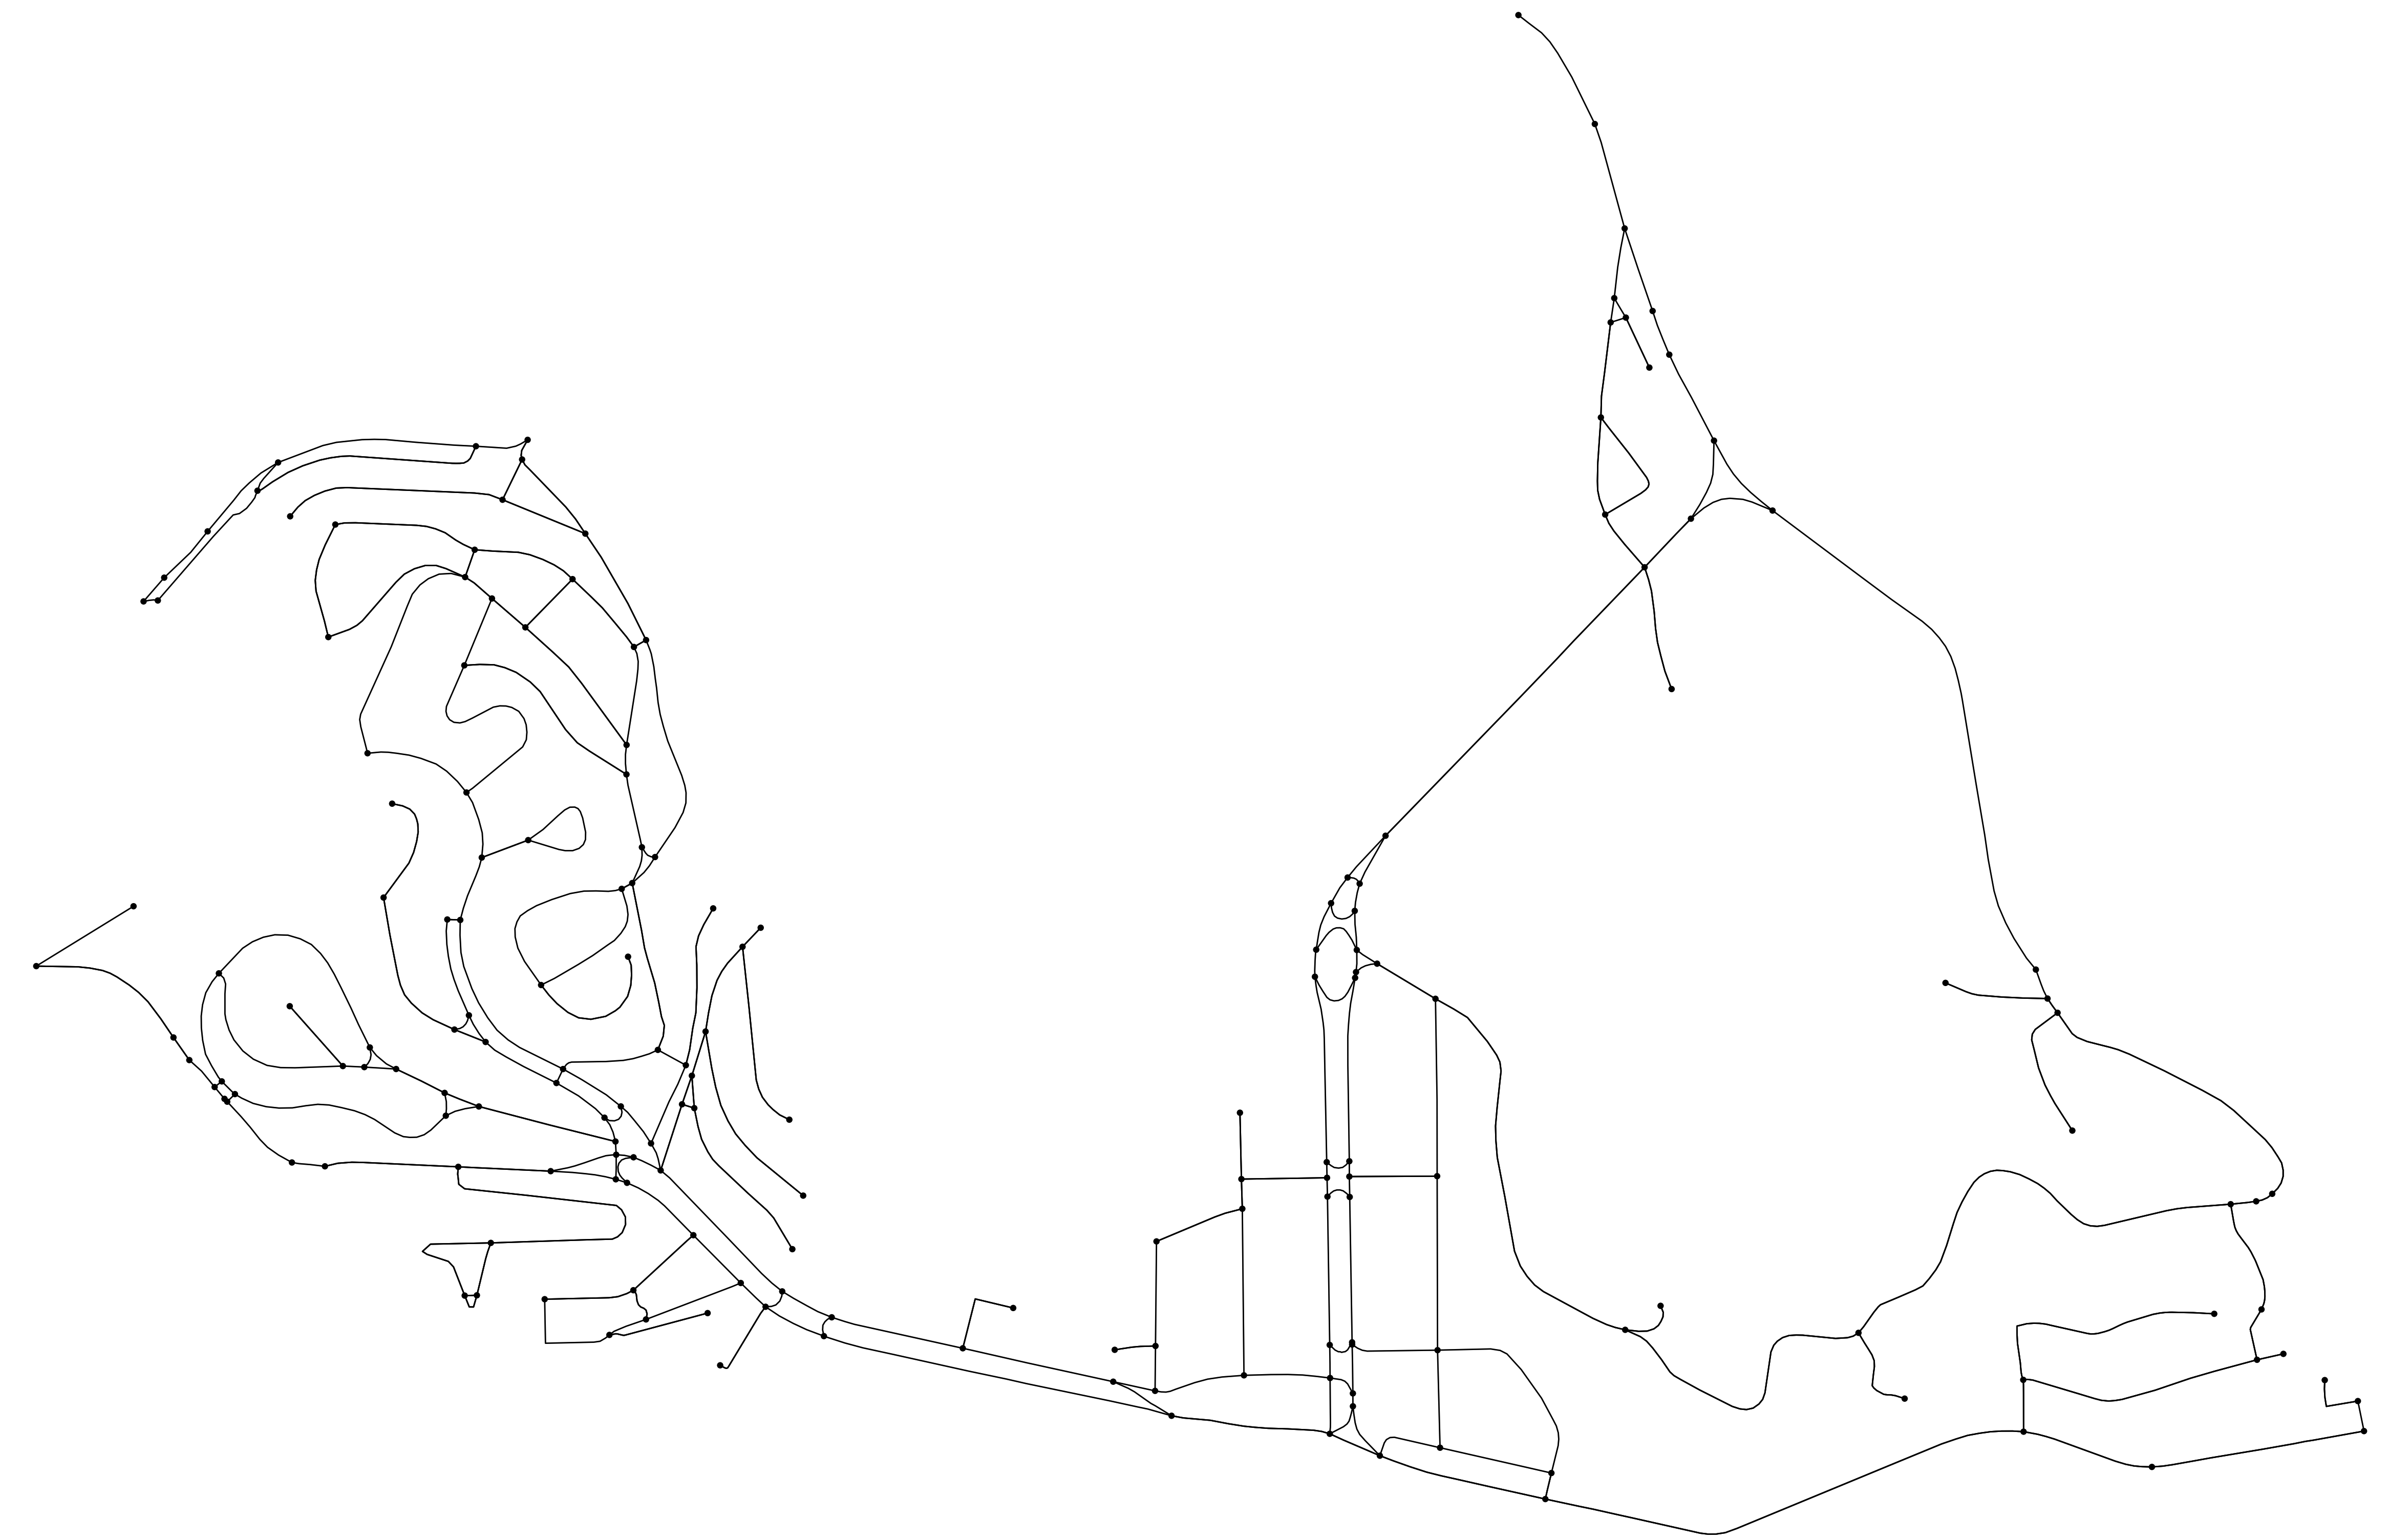
\includegraphics[width=\textwidth]{ondina_grafo_bruto}
    \caption{Visualização das ruas do bairro de Ondina com os vértices associados.}
    \label{fig:ondina_grafo_bruto}
\end{figure}

\subsection{Simplificação do Grafo}

Para adequar o grafo ao problema em análise, foi realizada uma simplificação que assumiu a existência de um campo de visão claro entre os nós conectados por uma aresta. Esta suposição eliminou obstáculos visuais e permitiu modelar de forma idealizada o problema, mantendo apenas os elementos essenciais para a análise.

O resultado do grafo simplificado é apresentado na Figura~\ref{fig:ondina_grafo_simplificado}, mostrando a estrutura final com as simplificações implementadas.

\begin{figure}[H]
    \centering
    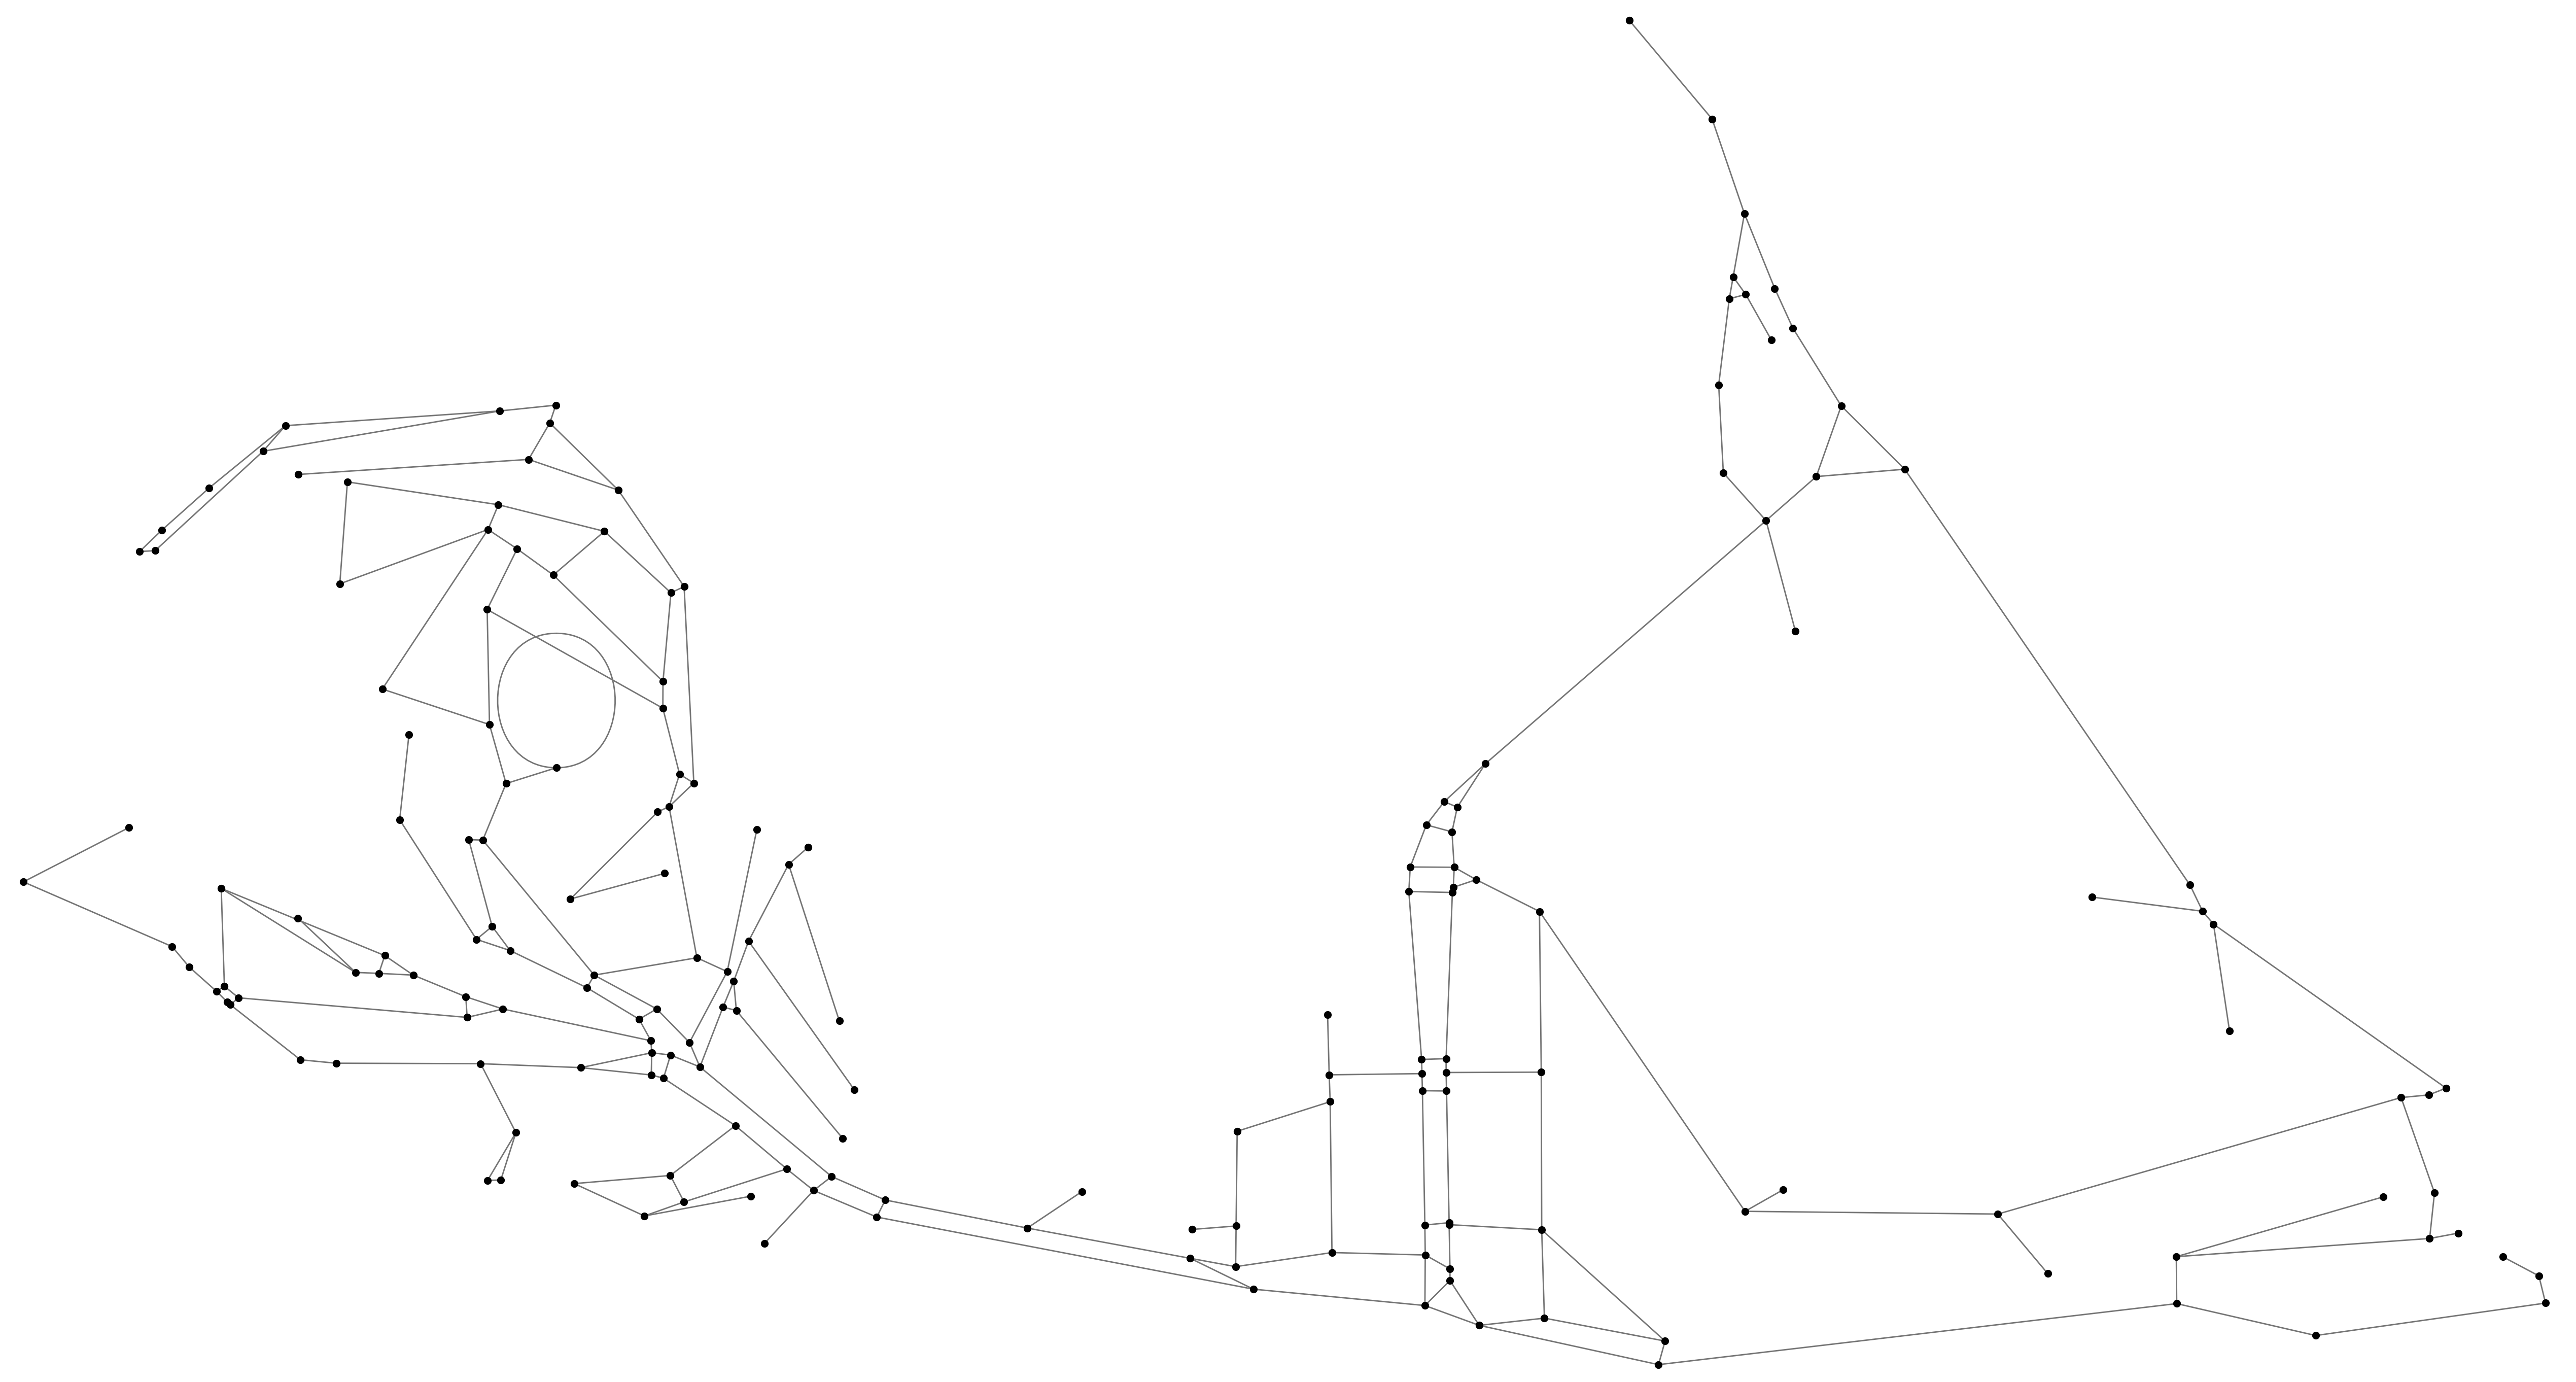
\includegraphics[width=\textwidth]{ondina_grafo_simplificado}
    \caption{Visualização do grafo simplificado do bairro de Ondina.}
    \label{fig:ondina_grafo_simplificado}
\end{figure}

\subsection{Discussão}

A simplificação realizada, ao assumir a existência de campo de visão claro entre os nós, possibilitou o uso do grafo para aplicações práticas no problema em análise. Essa abordagem é particularmente útil em cenários que envolvem monitoramento ou comunicação direta, como a análise de cobertura por câmeras, onde barreiras visuais poderiam ser tratadas como elementos externos ao modelo principal.

O processo de extração, construção e simplificação do grafo demonstra como é possível transformar dados geográficos brutos em representações abstratas otimizadas para resolver problemas específicos. A estrutura final do grafo oferece um modelo compacto e eficiente, adequado para o estudo da cobertura de vértices no contexto urbano de Ondina.

\subsection{Estrutura do Grafo}

O grafo é definido como um conjunto de \textbf{nós} e \textbf{arestas}, organizados da seguinte forma:

\begin{itemize}
    \item \textbf{Nós (Nodes):}
    Cada nó representa um ponto no mapa, definido por suas coordenadas geográficas:
    \begin{itemize}
        \item \texttt{id}: Identificador único do nó.
        \item \texttt{lat}: Latitude do ponto.
        \item \texttt{lon}: Longitude do ponto.
    \end{itemize}
    Exemplo de definição de nós:
\begin{verbatim}
{
  "id": 0,
  "lat": -13.000871,
  "lon": -38.5054976
},
{
  "id": 1,
  "lat": -13.0016275,
  "lon": -38.5057271
}
\end{verbatim}

    \item \textbf{Arestas (Edges):}
    As arestas conectam dois nós, representando ruas ou trechos que ligam os pontos geográficos. Cada aresta é caracterizada por:
    \begin{itemize}
        \item \texttt{source}: Identificador do nó de origem.
        \item \texttt{target}: Identificador do nó de destino.
        \item \texttt{weight}: Peso da aresta, que pode ser interpretado como a distância entre os dois pontos.
        \item \texttt{name}: Nome da rua ou caminho.
    \end{itemize}
    Exemplo de definição de arestas:
\begin{verbatim}
{
  "source": 0,
  "target": 3,
  "weight": 99.5182593770244,
  "name": "Avenida Anita Garibaldi"
},
{
  "source": 1,
  "target": 3,
  "weight": 96.76899596360965,
  "name": "Avenida Milton Santos"
}
\end{verbatim}
    \item \textbf{Metadados:}
    O grafo também inclui informações descritivas adicionais, como:
    \begin{itemize}
        \item \texttt{name}: Nome do grafo, neste caso, "Grafo de Ondina".
        \item \texttt{description}: Descrição geral, como "Grafo das ruas do bairro de Ondina, Salvador".
        \item \texttt{source}: Fonte dos dados, como "OpenStreetMap".
    \end{itemize}
\end{itemize}

\chapter{Solução Algorítmica}

\section{Pseudo-Código e Algoritmo Utilizado}
O algoritmo implementado para resolver o problema de cobertura de vértices utiliza duas abordagens principais: cobertura completa e cobertura máxima. Ambas são baseadas em uma estratégia gulosa (greedy) que seleciona iterativamente os vértices mais promissores.

\subsection{Algoritmo de Cobertura Completa}
O algoritmo de cobertura completa visa encontrar o menor conjunto de vértices que cubra todo o grafo. Abaixo está o pseudocódigo detalhado:

\begin{algorithm}[H]
\caption{Algoritmo de Cobertura Completa}
\begin{algorithmic}[1]
\State \textbf{Entrada:} Grafo G = (V, E)
\State \textbf{Saída:} Conjunto C de vértices selecionados para instalação de câmeras
\Statex
\State \textbf{Inicialização:}
\State vertices\_nao\_cobertos $\gets$ V
\State cobertura $\gets \emptyset$
\Statex
\While{vertices\_nao\_cobertos $\neq \emptyset$}
    \State melhor\_vertice $\gets$ null
    \State max\_cobertura $\gets$ 0
    \ForAll{v $\in$ V}
        \If{v $\notin$ cobertura}
            \State vizinhos $\gets$ N(v) $\cup$ \{v\} \Comment{N(v) são os vizinhos de v}
            \State cobertura\_atual $\gets$ |vizinhos $\cap$ vertices\_nao\_cobertos|
            \If{cobertura\_atual > max\_cobertura}
                \State max\_cobertura $\gets$ cobertura\_atual
                \State melhor\_vertice $\gets$ v
            \EndIf
        \EndIf
    \EndFor
    \If{melhor\_vertice = null}
        \State \textbf{break}
    \EndIf
    \State cobertura $\gets$ cobertura $\cup$ \{melhor\_vertice\}
    \State vertices\_nao\_cobertos $\gets$ vertices\_nao\_cobertos $\setminus$ (N(melhor\_vertice) $\cup$ \{melhor\_vertice\})
\EndWhile
\State \Return cobertura
\end{algorithmic}
\end{algorithm}

\subsection{Algoritmo de Cobertura Máxima}
O algoritmo de cobertura máxima busca maximizar a cobertura com um número limitado de câmeras:

\begin{algorithm}[H]
\caption{Algoritmo de Cobertura Máxima}
\begin{algorithmic}[1]
\State \textbf{Entrada:} Grafo G = (V, E), número máximo de câmeras p
\State \textbf{Saída:} Conjunto C de vértices selecionados e conjunto de vértices cobertos
\Statex
\State \textbf{Inicialização:}
\State cobertura $\gets \emptyset$
\State vertices\_cobertos $\gets \emptyset$
\Statex
\For{i = 1 \textbf{to} p}
    \State melhor\_vertice $\gets$ null
    \State max\_novos\_cobertos $\gets$ 0
    \ForAll{v $\in$ V}
        \If{v $\notin$ cobertura}
            \State vizinhos $\gets$ N(v) $\cup$ \{v\}
            \State novos\_cobertos $\gets$ |vizinhos $\setminus$ vertices\_cobertos|
            \If{novos\_cobertos > max\_novos\_cobertos}
                \State max\_novos\_cobertos $\gets$ novos\_cobertos
                \State melhor\_vertice $\gets$ v
            \EndIf
        \EndIf
    \EndFor
    \If{melhor\_vertice = null \textbf{or} max\_novos\_cobertos = 0}
        \State \textbf{break}
    \EndIf
    \State cobertura $\gets$ cobertura $\cup$ \{melhor\_vertice\}
    \State vertices\_cobertos $\gets$ vertices\_cobertos $\cup$ N(melhor\_vertice) $\cup$ \{melhor\_vertice\}
\EndFor
\State \Return (cobertura, vertices\_cobertos)
\end{algorithmic}
\end{algorithm}

\subsection{Complexidade Computacional}
A análise de complexidade dos algoritmos implementados é a seguinte:

\begin{itemize}
    \item \textbf{Cobertura Completa:}
    \begin{itemize}
        \item Tempo: O($\lvert V \rvert^2$), onde $\lvert V \rvert$ é o número de vértices no grafo
        \item Espaço: O($\lvert V \rvert$) para armazenar os conjuntos de vértices
        \item O loop principal executa no máximo $\lvert V \rvert$ vezes
        \item Para cada iteração, visitamos todos os vértices não cobertos
    \end{itemize}
    
    \item \textbf{Cobertura Máxima:}
    \begin{itemize}
        \item Tempo: O(p$\lvert V \rvert$), onde p é o número máximo de câmeras
        \item Espaço: O($\lvert V \rvert$) para armazenar os conjuntos de vértices
        \item O loop principal executa exatamente p vezes
        \item Para cada iteração, visitamos todos os vértices não selecionados
    \end{itemize}
\end{itemize}

\subsection{Implementação}
A implementação foi realizada em Python utilizando a biblioteca NetworkX para manipulação de grafos. A classe \texttt{CoberturaVertices} encapsula toda a lógica dos algoritmos:

\begin{itemize}
    \item \textbf{Estruturas de Dados:}
    \begin{itemize}
        \item Grafo representado como objeto \texttt{nx.Graph}
        \item Matriz de adjacência para acesso rápido às conexões
        \item Conjuntos para rastreamento de vértices cobertos/não cobertos
    \end{itemize}
    
    \item \textbf{Principais Métodos:}
    \begin{itemize}
        \item \texttt{resolve\_cobertura\_completa()}: Implementa o algoritmo de cobertura completa
        \item \texttt{resolve\_cobertura\_maxima(p)}: Implementa o algoritmo de cobertura máxima
        \item \texttt{salvar\_resultado()}: Persiste os resultados em formato JSON
    \end{itemize}
    
    \item \textbf{Otimizações:}
    \begin{itemize}
        \item Uso de estruturas de dados eficientes (sets) para operações de união e interseção
        \item Cálculo incremental de coberturas para evitar recomputação
        \item Armazenamento em cache da matriz de adjacência
    \end{itemize}
\end{itemize}

Os resultados são salvos em arquivos JSON contendo:
\begin{itemize}
    \item Lista de vértices selecionados para instalação de câmeras
    \item Número total de câmeras utilizadas
    \item Cobertura total alcançada (número de vértices cobertos)
    \item Total de vértices no grafo
\end{itemize}

Esta implementação está disponível no arquivo \texttt{5\_resolve\_cobertura.py} e pode ser executada após a geração do grafo inicial do bairro de Ondina.

\chapter{Experimentos}

\section{Metodologia}
\subsection{Instâncias}
Os dados utilizados nos experimentos foram extraídos do OpenStreetMap, representando o bairro de Ondina. Os pontos potenciais para câmeras foram identificados com base na estrutura viária.

\chapter{Considerações Finais}

\section{Conclusão}
O projeto demonstrou a aplicabilidade da teoria dos grafos na solução de problemas reais de segurança pública. A abordagem de cobertura de vértices mostrou-se eficiente e prática, oferecendo uma solução otimizada para o posicionamento de câmeras no bairro de Ondina.

%-------------Bibliografia------------------
\newpage
\renewcommand{\refname}{Referências Bibliográficas}
\addcontentsline{toc}{chapter}{Referências Bibliográficas}
\bibliography{Bibliografia}
\nocite{*}

\end{document}